\documentclass[11pt,a4paper]{article}
\usepackage[utf8]{inputenc}
\usepackage[margin=1in]{geometry}
\usepackage{amsmath,amssymb}
\usepackage{graphicx}
\usepackage{xcolor}
\usepackage{booktabs}
\usepackage{array}
\usepackage{hyperref}
\usepackage{fancyhdr}
\usepackage{enumitem}
\usepackage{titlesec}
\usepackage{caption}

% Color Palette
\definecolor{primary}{RGB}{31, 78, 121}
\definecolor{secondary}{RGB}{41, 128, 185}
\definecolor{darktext}{RGB}{44, 62, 80}

\hypersetup{
    colorlinks=true,
    linkcolor=secondary,
    citecolor=secondary,
    urlcolor=secondary
}

\pagestyle{fancy}
\fancyhf{}
\rhead{\textcolor{secondary}{\small HealthConnect ML Problem Definition \& System Design}}
\lhead{\textcolor{secondary}{\small AnalystLab Africa — Week 4}}
\rfoot{\textcolor{secondary}{\small Page \thepage}}
\lfoot{\textcolor{secondary}{\small Intern: Rudolf (ML Track)}}

\titleformat{\section}{\Large\bfseries\color{primary}}{\thesection}{1em}{}
\titleformat{\subsection}{\large\bfseries\color{secondary}}{\thesubsection}{1em}{}

\begin{document}

% Title Page
\begin{titlepage}
\centering
\vspace*{1cm}
{\huge\bfseries\color{primary} ANALYSTLAB AFRICA INTERNSHIP PROGRAMME\par}
\vspace{0.5cm}
{\Large\bfseries\color{secondary} HealthConnect Experience Lab — Week 4 Kickoff\par}
\vspace{1.5cm}

\rule{\linewidth}{1.5pt}\\[0.4cm]
{\huge \bfseries Machine Learning Problem Definition \& Production System Design Report}\\[0.4cm]
\rule{\linewidth}{1.5pt}\\[1.5cm]

\begin{minipage}{0.48\textwidth}
\begin{flushleft} \large
\textbf{Intern Name:} Rudolf\\
\textbf{Track:} Machine Learning Engineering / Data Science\\
\textbf{Role:} Junior Machine Learning Engineer\\
\textbf{Date:} August 2026
\end{flushleft}
\end{minipage}
\begin{minipage}{0.48\textwidth}
\begin{flushright} \large
\textbf{Project:} HealthConnect Clinic\\
\textbf{Document Version:} 1.0\\
\textbf{Status:} Kickoff Deliverable\\
\textbf{Mentor Access:} Granted
\end{flushright}
\end{minipage}

\vfill
\begin{abstract}
\noindent This document establishes the foundational Machine Learning Problem Definition and Production System Architecture for the HealthConnect Clinic Experience Lab. Facing high non-attendance rates ($48.46\%$ baseline no-show rate), HealthConnect Clinic requires an automated, predictive, and actionable system to mitigate appointment missed slots, optimize provider schedule utilization, and improve patient support. We formulate a supervised binary classification task $P(\text{No-Show} \mid X)$, evaluate data quality across 5,000 appointment records, present a candidate feature taxonomy across 6 domain categories, define strict data leakage boundaries, and detail an end-to-end production ML system design incorporating real-time inference microservices, automated multi-channel intervention workflows, MLOps monitoring, and HIPAA-compliant governance.
\end{abstract}

\vfill
\end{titlepage}

\newpage
\tableofcontents
\newpage

% Section 1
\section{Executive Summary \& Project Context}
\subsection{Business Scenario}
HealthConnect Clinic is an outpatient healthcare provider managing appointment-based clinical consultation and diagnostic services. The clinic suffers from severe operational bottlenecks driven by patient appointment non-attendance. When patients miss scheduled appointments without prior notice, clinical capacity remains idle, patient care continuity is disrupted, and healthcare overhead escalates.

\subsection{Central Project Question}
\begin{quote}
\textit{How can HealthConnect Clinic leverage data, machine learning, and Generative AI to accurately predict appointment no-shows, deliver proactive patient engagement, and maximize clinical slot utilization?}
\end{quote}

\subsection{Project Transition \& Week 4 Scope}
During Weeks 1--3, foundational data manipulation and classification modeling techniques were executed on telecom churn data. Beginning in Week 4, the internship transitions to the HealthConnect Experience Lab. Week 4 serves as the critical problem formulation and architectural design phase.

---

% Section 2
\section{Comprehensive Data Quality \& Suitability Assessment}
\subsection{Dataset Overview}
The primary analytical resource is \texttt{HealthConnect\_Appointment\_Data.csv}, containing $5,000$ synthetic anonymized appointment records across $1,696$ unique patients (\texttt{patient\_id}).

\begin{table}[h!]
\centering
\caption{HealthConnect Dataset Variable Breakdown \& Missingness Profile}
\label{tab:data_dict}
\small
\begin{tabular}{lllll}
\toprule
\textbf{Variable Name} & \textbf{Data Type} & \textbf{Missing Count (\%)} & \textbf{Role in ML Pipeline} & \textbf{Notes / Mechanism} \\
\midrule
\texttt{appointment\_id} & String & 0 (0.0\%) & Primary Key & Excluded from modeling \\
\texttt{patient\_id} & String & 0 (0.0\%) & Grouping Key & Used for GroupKFold split \\
\texttt{gender} & Categorical & 0 (0.0\%) & Feature & Female, Male, Prefer not to say \\
\texttt{age} & Integer & 0 (0.0\%) & Feature & Range: 18--80 years \\
\texttt{age\_group} & Categorical & 0 (0.0\%) & Feature & 6 derived age bands \\
\texttt{appointment\_type} & Categorical & 0 (0.0\%) & Feature & 4 appointment categories \\
\texttt{booking\_date} & Datetime & 0 (0.0\%) & Temporal & Lead time computation \\
\texttt{appointment\_date} & Datetime & 0 (0.0\%) & Temporal & Target schedule date \\
\texttt{appointment\_day} & Categorical & 0 (0.0\%) & Feature & Day of week \\
\texttt{appointment\_time} & Categorical & 0 (0.0\%) & Feature & Morning, Afternoon, Evening \\
\texttt{booking\_lead\_days} & Integer & 0 (0.0\%) & Feature & Days between booking \& appt \\
\texttt{previous\_appointments} & Integer & 0 (0.0\%) & Feature & Patient historical count \\
\texttt{previous\_no\_shows} & Integer & 0 (0.0\%) & Feature & Patient historical no-shows \\
\texttt{reminder\_sent} & Categorical & 0 (0.0\%) & Feature & Binary (Yes / No) \\
\texttt{reminder\_channel} & Categorical & 1,366 (27.3\%) & Feature & NMAR (Missing when Sent=No) \\
\texttt{distance\_to\_clinic\_km} & Float & 90 (1.8\%) & Feature & MCAR (Median Imputation) \\
\texttt{waiting\_time\_minutes} & Float & 60 (1.2\%) & Excluded & MAR (Data Leakage Risk!) \\
\texttt{appointment\_outcome} & Categorical & 0 (0.0\%) & Target Source & Attended, No-Show, Cancelled \\
\bottomrule
\end{tabular}
\end{table}

\subsection{Target Outcome Class Distribution}
Analysis of \texttt{appointment\_outcome} across the $5,000$ records reveals:
\begin{itemize}
    \item \textbf{No-Show:} 2,423 records ($48.46\%$)
    \item \textbf{Attended:} 2,314 records ($46.28\%$)
    \item \textbf{Cancelled:} 263 records ($5.26\%$)
\end{itemize}

\subsection{Missing Value Mechanisms \& Preprocessing Strategy}
\begin{enumerate}
    \item \textbf{\texttt{reminder\_channel} (27.32\% Missing):} Not Missing At Random (NMAR). Missing values correspond exactly to appointments where no reminder was dispatched. Imputation strategy: assign explicit category \texttt{"None\_Sent"}.
    \item \textbf{\texttt{distance\_to\_clinic\_km} (1.80\% Missing):} Missing Completely At Random (MCAR). Imputation strategy: Group-median imputation by patient postal region / age group.
    \item \textbf{\texttt{waiting\_time\_minutes} (1.20\% Missing):} Data Leakage Safeguard. Because waiting time is measured post-arrival, utilizing it prior to appointment execution would introduce severe target leakage. Excluded entirely from training features.
\end{enumerate}

\subsection{Longitudinal Structure \& Cross-Validation Grouping}
The 5,000 appointments span 1,696 unique patients (average 2.95 appointments/patient). Standard random K-Fold cross-validation would leak individual patient behavioral traits between training and validation splits. Therefore, model validation must employ \textbf{GroupKFold CV} grouped by \texttt{patient\_id} or a strict \textbf{Temporal Train-Test Split} based on \texttt{booking\_date}.

---

% Section 3
\section{Machine Learning Problem Definition \& Formulation}
\subsection{Supervised Binary Classification Framing}
We frame the appointment attendance prediction task as a supervised binary classification problem. For each scheduled appointment $i$, we predict the probability of non-attendance:
\begin{equation}
P(Y_i = 1 \mid X_i) = \sigma(f(X_i))
\end{equation}
where $Y_i = 1$ if the appointment results in a \textbf{No-Show}, $Y_i = 0$ if \textbf{Attended}, and $X_i$ represents the vector of pre-appointment features available $T-48$ hours prior to schedule time.

\subsection{Operational Handling of Cancellations}
\texttt{Cancelled} appointments ($5.26\%$) are filtered out during model training. Operationally:
\begin{itemize}
    \item \textbf{Cancellations} reflect proactive patient communication, enabling clinic reception to rebook the open slot immediately.
    \item \textbf{No-Shows} reflect unannounced absences resulting in unrecoverable idle clinician capacity.
\end{itemize}
Hence, the primary ML system targets binary discrimination between Attended ($Y=0$) and No-Show ($Y=1$).

\subsection{Proposed Candidate Feature Taxonomy}
\begin{enumerate}
    \item \textbf{Patient Demographics:} \texttt{age}, \texttt{gender}, \texttt{age\_group}.
    \item \textbf{Appointment Attributes:} \texttt{appointment\_type}, \texttt{appointment\_day}, \texttt{appointment\_time}.
    \item \textbf{Temporal \& Lead Time Metrics:} \texttt{booking\_lead\_days}, lead time binned windows (\texttt{0-3d}, \texttt{4-7d}, \texttt{8-14d}, \texttt{15-30d}, \texttt{31-60d}, \texttt{60d+}).
    \item \textbf{Historical Behavioral Signals:} \texttt{previous\_appointments}, \texttt{previous\_no\_shows}, engineered feature $\text{\texttt{historical\_noshow\_ratio}} = \frac{\texttt{previous\_no\_shows}}{\max(\texttt{previous\_appointments}, 1)}$.
    \item \textbf{Communication Channels:} \texttt{reminder\_sent}, \texttt{reminder\_channel} (\texttt{SMS}, \texttt{WhatsApp}, \texttt{Email}, \texttt{None\_Sent}).
    \item \textbf{Geographical Logistics:} \texttt{distance\_to\_clinic\_km}.
\end{enumerate}

---

% Section 4
\section{End-to-End Production Machine Learning System Design}
\subsection{High-Level System Architecture}
The production ML prediction platform consists of five modular microservices:

\begin{figure}[h!]
\centering
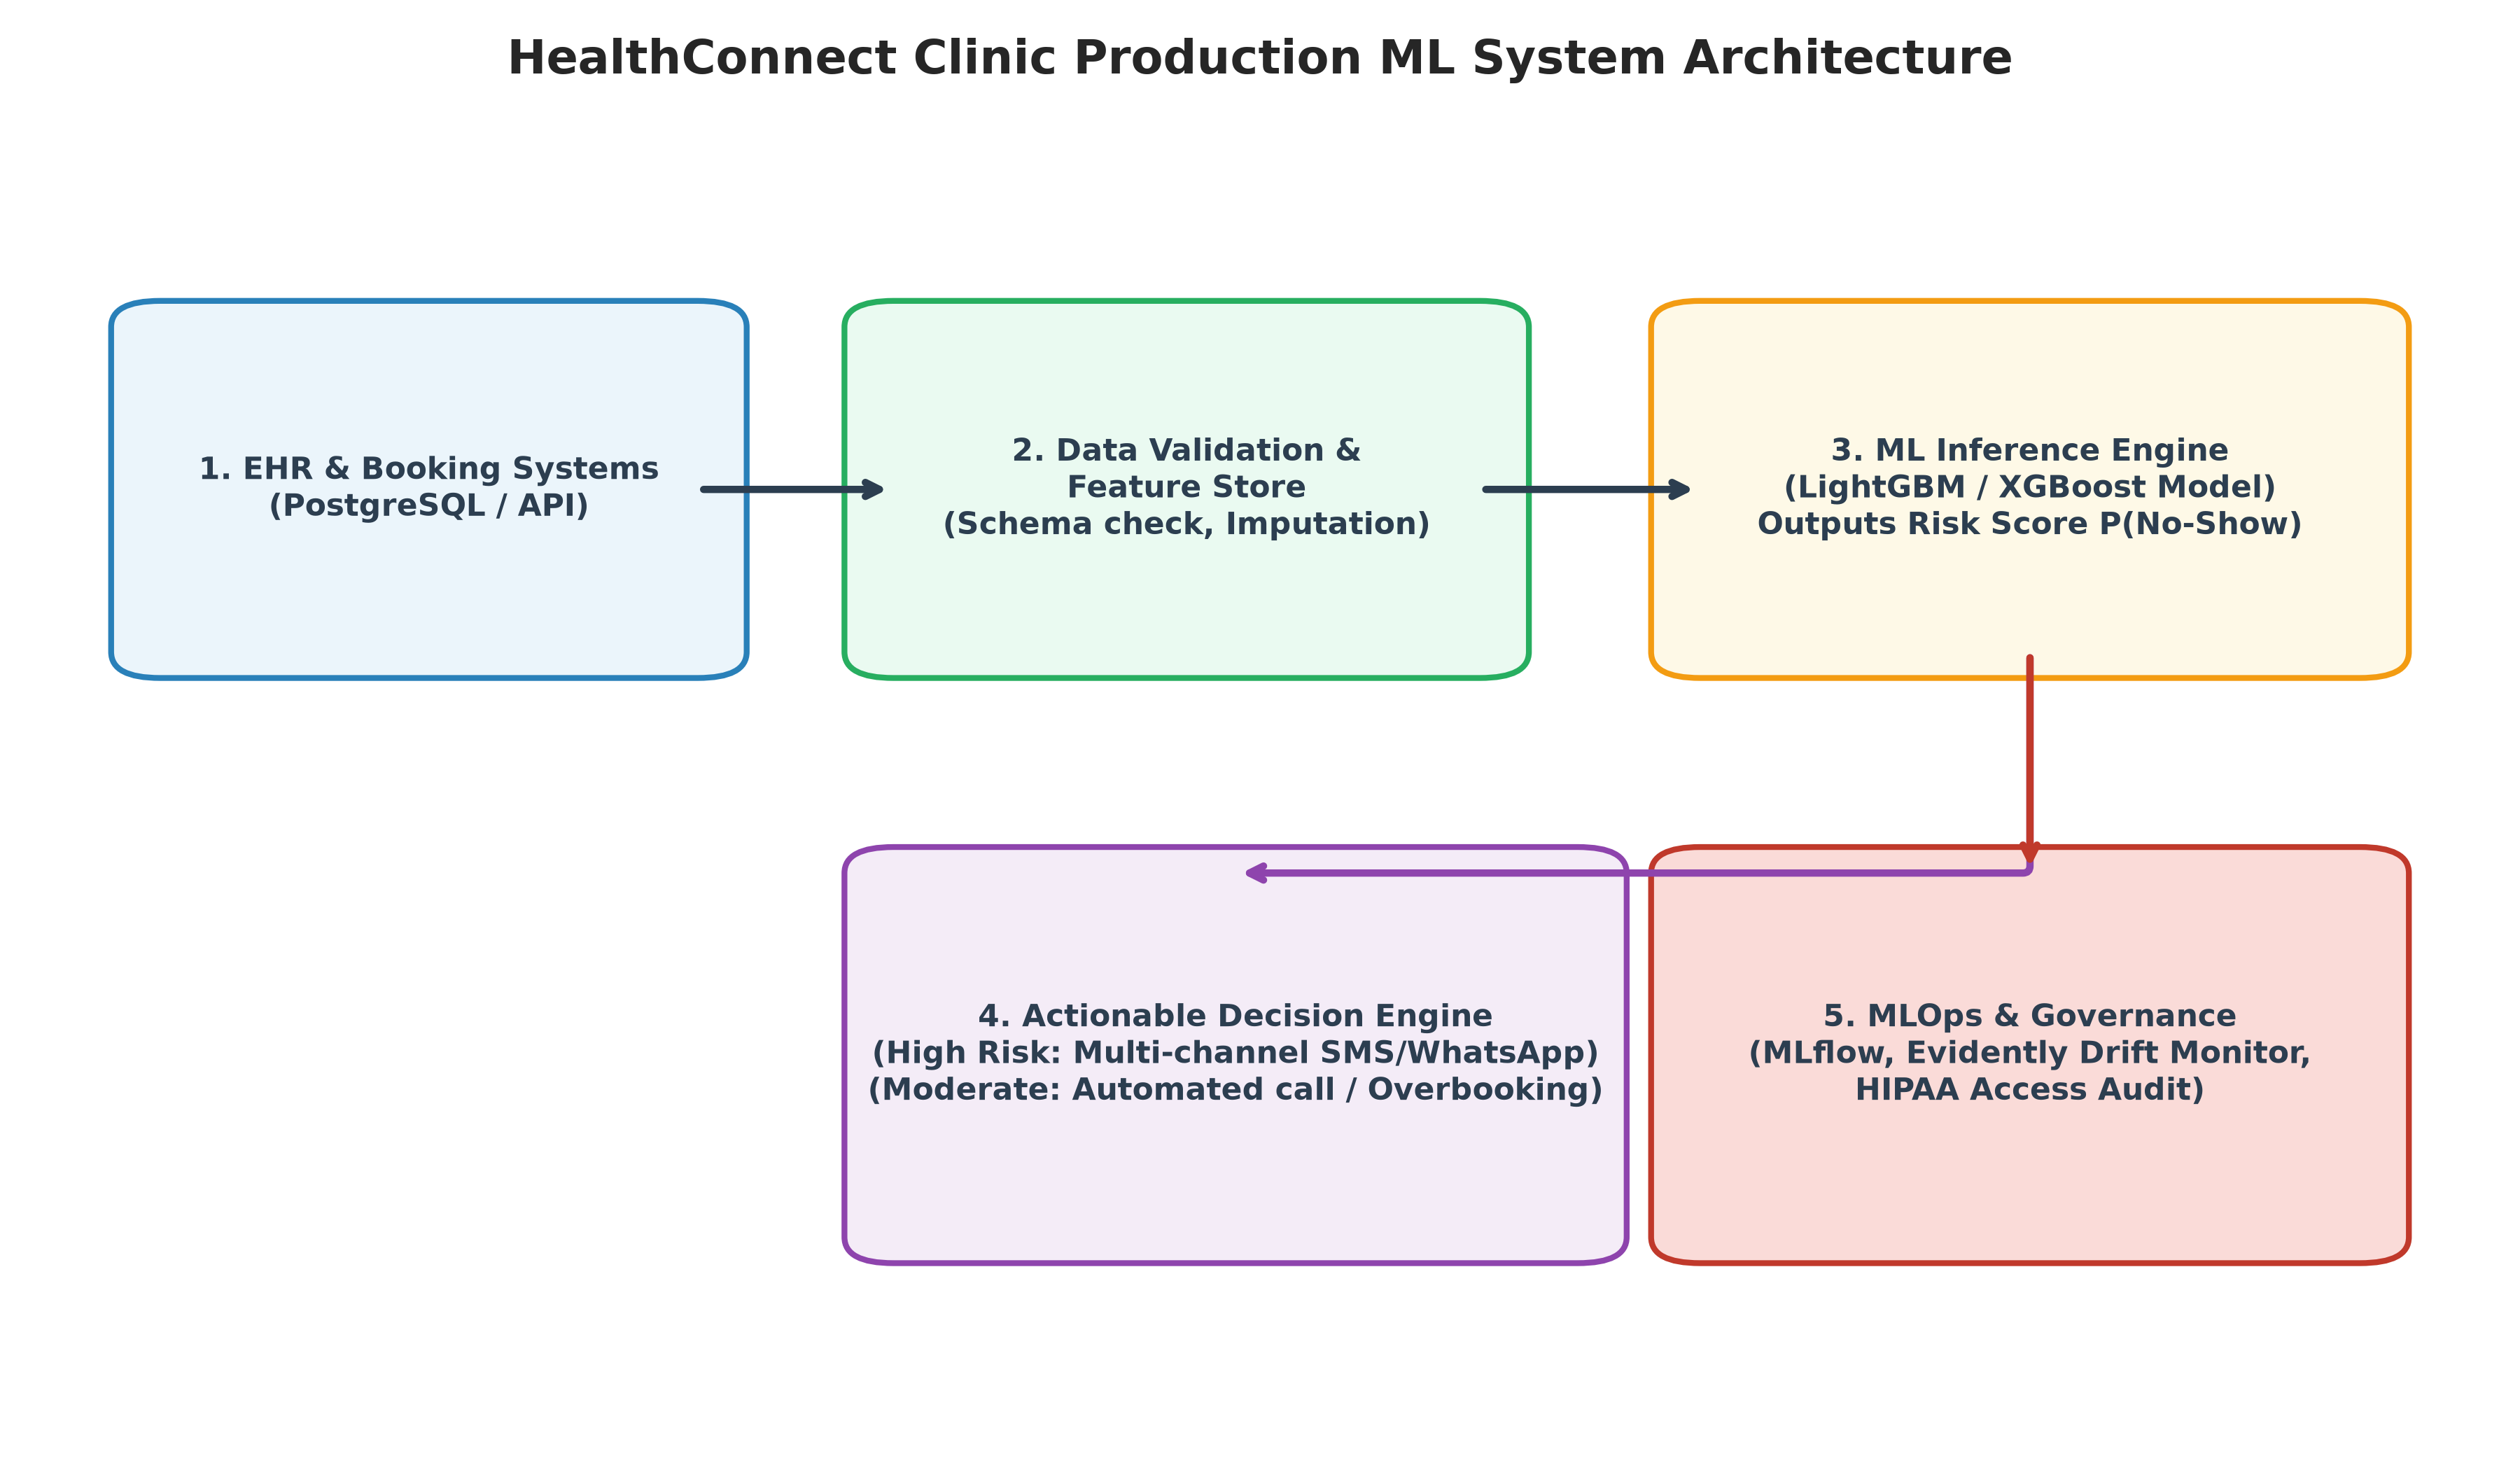
\includegraphics[width=0.95\linewidth]{../figures/fig05_system_architecture.png}
\caption{Production Machine Learning System Architecture for HealthConnect Clinic}
\label{fig:arch}
\end{figure}

\begin{enumerate}
    \item \textbf{EHR Ingestion Pipeline:} Synchronizes upcoming appointments daily from PostgreSQL EHR database $T-48$ hours prior to scheduled date.
    \item \textbf{Feature Store \& Schema Validator:} Validates data schema using Great Expectations, imputes missing values, and fetches historical patient aggregations.
    \item \textbf{ML Inference Service:} Containerized FastAPI service serving calibrated LightGBM / XGBoost models, returning $P(\text{No-Show})$.
    \item \textbf{Actionable Decision Engine:} Classifies risk tier and triggers automated patient engagement:
    \begin{itemize}
        \item \textbf{High Risk ($P > 0.70$):} Multi-channel SMS + WhatsApp interactive confirmation; flag slot for standby buffer overbooking.
        \item \textbf{Moderate Risk ($0.40 \le P \le 0.70$):} Automated SMS reminder requesting 1-click confirmation or rescheduling.
        \item \textbf{Low Risk ($P < 0.40$):} Standard single email notification.
    \end{itemize}
    \item \textbf{MLOps \& Drift Monitoring:} Logs inputs, predictions, and actual outcomes to MLflow registry and Prometheus/Grafana dashboards.
\end{enumerate}

\subsection{API Schema Specifications}
\textbf{Request Payload (\texttt{POST /v1/predict-noshow}):}
\begin{verbatim}
{
  "appointment_id": "HC-00412",
  "patient_id": "P-0912",
  "age": 42,
  "gender": "Female",
  "appointment_type": "Specialist Consultation",
  "booking_lead_days": 18,
  "previous_appointments": 4,
  "previous_no_shows": 2,
  "reminder_sent": "Yes",
  "reminder_channel": "SMS",
  "distance_to_clinic_km": 14.2
}
\end{verbatim}

\textbf{Response Payload:}
\begin{verbatim}
{
  "appointment_id": "HC-00412",
  "no_show_probability": 0.764,
  "risk_tier": "HIGH_RISK",
  "recommended_action": "TRIGGER_WHATSAPP_CONFIRMATION_AND_BUFFERSLOT",
  "model_version": "v1.2.0-lightgbm"
}
\end{verbatim}

---

% Section 5
\section{Reproducibility, MLOps, Governance \& Ethics}
\subsection{Reproducibility Framework}
All model artifacts, hyperparameters, pipelines, and evaluation metrics will be version-controlled via DVC (Data Version Control) and tracked using MLflow. Code repositories maintain deterministic random seeds across data splitting, imputation, and model training routines.

\subsection{Model Governance \& Monitoring}
\begin{itemize}
    \item \textbf{Data Drift Monitoring:} Statistical Kolmogorov-Smirnov tests executed weekly via Evidently AI to detect feature drift in \texttt{booking\_lead\_days} or demographic shifts.
    \item \textbf{Concept Drift Monitoring:} Performance metrics (Recall, ROC-AUC, Log-Loss) evaluated weekly against actual attendance logs.
\end{itemize}

\subsection{Ethical Considerations \& Fairness}
Healthcare predictive models must avoid systemic bias against vulnerable populations. Models will be evaluated for equalized odds and equal opportunity across demographic sub-groups (\texttt{age\_group}, \texttt{gender}, geographical distance). Interventions are non-punitive, providing extra engagement support rather than denying service.

---

% Section 6
\section{Assumptions, Limitations, Risks \& Next Steps}
\subsection{Risk Matrix}

\begin{table}[h!]
\centering
\caption{Project Risk Matrix \& Mitigation Strategy}
\label{tab:risk_matrix}
\small
\begin{tabular}{lp{3.5cm}llp{4.5cm}}
\toprule
\textbf{Risk Event} & \textbf{Description} & \textbf{Severity} & \textbf{Probability} & \textbf{Mitigation Strategy} \\
\midrule
Data Leakage & Post-arrival feature included in pre-appointment model & High & Medium & Exclude \texttt{waiting\_time\_minutes}; audit feature store pipelines. \\
Target Drift & Post-COVID patient behavior alters attendance patterns & High & Medium & Automated weekly drift detection \& bi-monthly model retraining. \\
Class Imbalance & Skewed outcome distributions across specialist clinics & Medium & Low & Cost-sensitive threshold tuning ($F_{\beta}$ optimization with $\beta=2$). \\
Cold Start & New patients lacking historical appointment records & Medium & High & Population prior imputation + lead time baseline weighting. \\
\bottomrule
\end{tabular}
\end{table}

\subsection{Proposed Focus for Week 5}
\begin{enumerate}
    \item Construct modular scikit-learn feature preprocessing pipelines (One-Hot Encoding, Robust Scaling, Imputation).
    \item Engineer behavioral interaction terms (\texttt{noshow\_ratio}, \texttt{lead\_time\_weeks}).
    \item Train and benchmark 5 baseline classifiers: Logistic Regression, Decision Trees, Random Forest, Gradient Boosting, LightGBM.
    \item Evaluate performance on recall-focused metrics ($F_2$-score, ROC-AUC, PR-AUC).
\end{enumerate}

\end{document}
